\section{Introduction}
\subsection{Introduction}
The concept of smart homes has gained significant attention in recent years due to advancements in IoT technology. A smart home incorporates various devices and sensors that are interconnected and can be remotely monitored and controlled. This technology offers convenience, energy efficiency, and enhanced security to homeowners.

\begin{figure}[htbp]
    \centering
    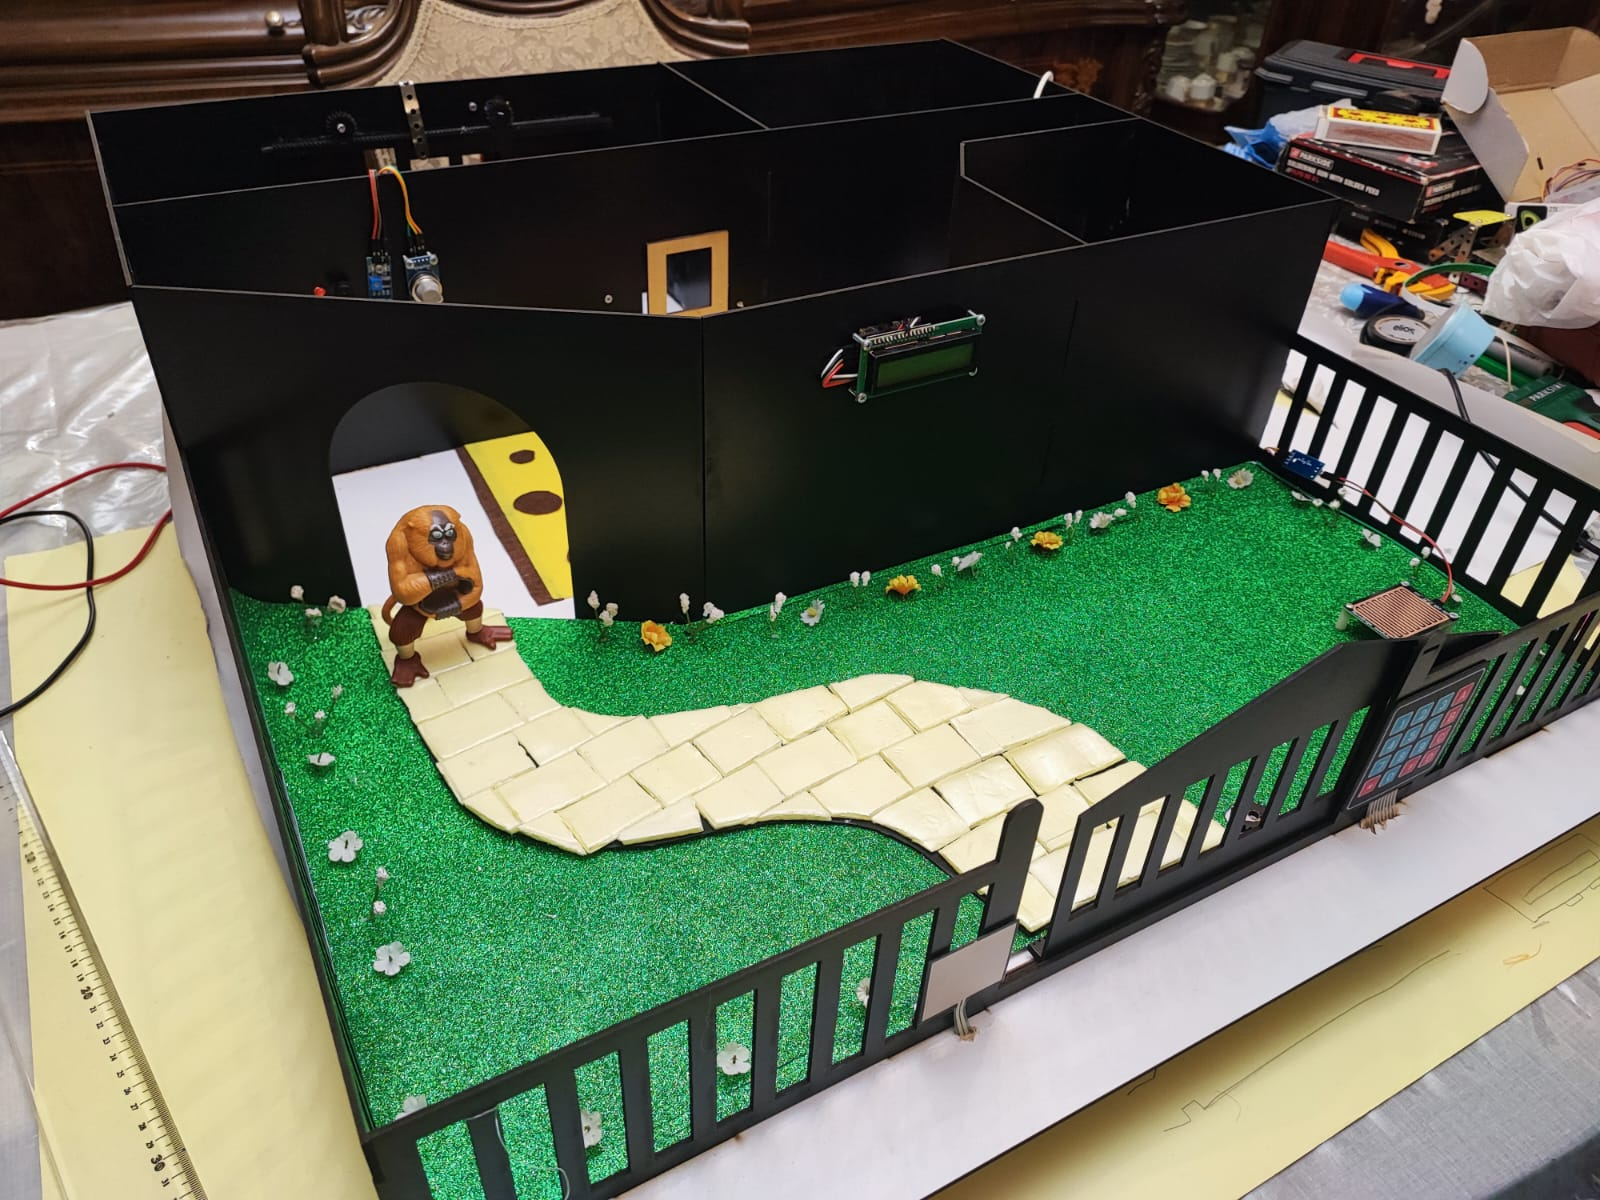
\includegraphics[width=0.8\textwidth]{figs/Smarthome1.jpg}
    \caption{Architecture of the smart home IoT project}
    \label{fig:architecture}
\end{figure}

\subsection{Motivation}
Our motivation for this project stems from the increasing demand for smart home solutions that offer convenience, energy efficiency, and security to homeowners.

\subsection{Problem Statement}
Despite the availability of various smart home solutions in the market, many of them lack customization options and integration capabilities. Our project aims to address these limitations by providing a customizable and integrated smart home solution.

\subsection{Objective}
The objective of our project is to develop a smart home IoT system that utilizes an ESP32 microcontroller and a mobile application for remote control and monitoring. 

\subsection{Project Features}
Key features of our smart home IoT project include:
\begin{itemize}
    \item Remote control and monitoring via a mobile application.
    \item Integration with various sensors and actuators for environmental monitoring and control.
    \item Enhanced security features such as door/window monitoring and intrusion detection and an alarm system.
    \item Rain System
    \item Smart Monitoring System
    \item Smart Light System
\end{itemize}

\subsection{System Requirements}
\subsubsection{Hardware Requirements}
The hardware requirements for our smart home IoT project include:

\begin{itemize}
    \item \textbf{ESP32 microcontroller}
    \begin{tabular}{cccc}
        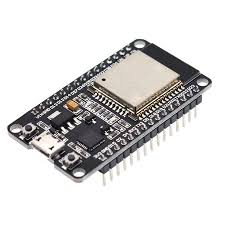
\includegraphics[width=0.15\textwidth]{figs/esp.png} \\
        ESP32 Mircocontroller \\
    \end{tabular}
    
    \item \textbf{Sensors:}
    
    \begin{tabular}{cccc}
        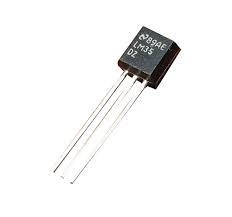
\includegraphics[width=0.15\textwidth]{figs/temp.png} &
        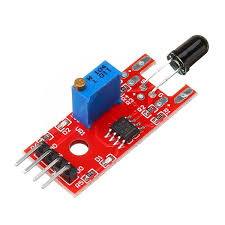
\includegraphics[width=0.15\textwidth]{figs/flame.png} &
        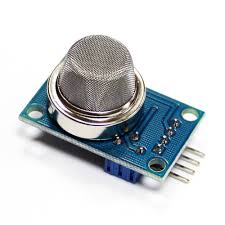
\includegraphics[width=0.15\textwidth]{figs/smoke.png} &
        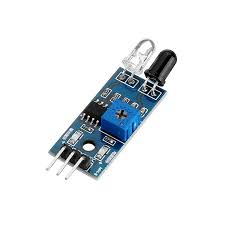
\includegraphics[width=0.15\textwidth]{figs/ir.png} \\
        
        Temperature Sensor & Flame Sensor & Smoke Sensor & Motion Sensor \\
        
        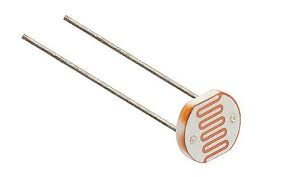
\includegraphics[width=0.15\textwidth]{figs/ldr.png} \\        
        Light Sensor \\
    \end{tabular}

    \item \textbf{Actuators:}
    
    \begin{tabular}{cccc}
        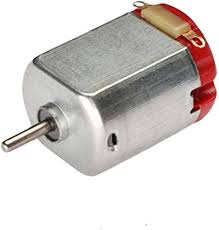
\includegraphics[width=0.20\textwidth]{figs/motor.png} &
        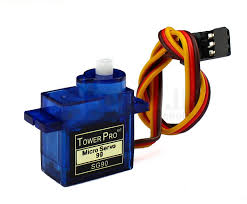
\includegraphics[width=0.20\textwidth]{figs/servo.png} &
        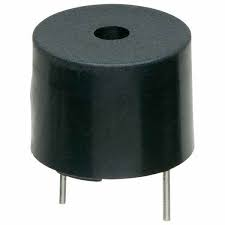
\includegraphics[width=0.20\textwidth]{figs/buzzer.png}\\
        
        DC Motor & Servo Motor & Buzzer 3\\
    \end{tabular}
\end{itemize}



\subsubsection{Software Requirements}
The software requirements for our smart home IoT project include:
\begin{itemize}
    \item Arduino IDE for programming the ESP32 microcontroller.
    \item Mobile application development framework (e.g., Flutter) for developing the mobile application.
    \item Communication protocols (e.g., MQTT) for data exchange between devices.
    \item Database management system (e.g., Firebase) for storing user data and configurations.
\end{itemize}
